\documentclass[aps,reprint]{revtex4-2}
\usepackage{listings}
\usepackage{graphicx}
\usepackage{float}
\usepackage{lipsum}
\usepackage[spanish]{babel}
\usepackage{amsmath}
\usepackage{amssymb}
\usepackage{booktabs}
\usepackage{xcolor}
\usepackage{listings}
\usepackage{longtable}
\lstset{
	language = R,
  backgroundcolor=\color{gray!5},    % very light gray background
  basicstyle=\ttfamily\small,        % monospaced font, small size
  frame=single,                      % adds a border around the code
  rulecolor=\color{gray!40},         % border color
  tabsize=2,                         % tab width
  showstringspaces=false,            % don't show spaces in strings
  breaklines=true,                   % line breaking
  breakatwhitespace=true,            % break only at white space
  numbers=left,                      % line numbers on the left
  numberstyle=\tiny\color{gray!70},  % line number style
  numbersep=6pt,                     % distance from numbers to code
  keywordstyle=\color{blue!70!black}\bfseries, % keywords in blue and bold
  commentstyle=\color{green!40!black}\itshape, % comments in green italic
  stringstyle=\color{orange!70!black},          % strings in orange
  identifierstyle=\color{black},     % normal text
  captionpos=b,                      % caption below
  keepspaces=true,                   % keep spaces in text
  escapeinside={(*@}{@*)},           % for LaTeX within code
  literate={~}{{\textasciitilde}}1   % fix tilde display
}

\begin{document}
\title{Análisis inferencial del vínculo entre estímulos lectores en la infancia y hábitos de lectura en la adultez: evidencia del MOLEC-INEGI 2020}
\author{A. Eduardo Luna\\Rafael Sánchez\\Sebastián Cortés\\ Emilio Alonso Sánchez\\github.com/Lunaaaalj/MEPTD}
\date{\today}
\affiliation{Instituto Tecnológico y de Estudios Superiores de Monterey}

\begin{abstract}
    En el presente trabajo se analiza el impacto que tienen los estímulos de lectura en la infancia sobre el desarrollo del hábito lector en la vida adulta, utilizamos datos del módulo sobre la lectura (MOLEC) el cual es generado por el INEGI, la problemática que utilizamos también es la desigualdad de oportunidades al acceso de materiales durante la niñez, la propuesta fue que el entorno familiar y cultural tienen mayor peso que la propia educación formal en la formación de lectores por gusto.

	Utilizamos técnicas estadísticas descriptivas e inferenciales para poder responder a nuestra pregunta de investigación, en la etapa de descripción encontramos las características principales de las variables demo gráficas, de estímulo y de hábito lector, pero en la etapa inferencial realizamos las pruebas de hipótesis con intervalos de confianza para determinar cuál es el impacto que tienen los estímulos infantiles en la lectura adulta. 
	
	Los resultados que obtuvimos confirman nuestra hipótesis planteada en la etapa 1, la cual se centra en que si los adultos fueron expuestos a practicas de lectura durante la infancia, tales como ver a los padres leer, si fueron a bibliotecas o tener libros en casa, estos presentan más probabilidad de leer en la actualidad, pero no encontramos grandes diferencias analizando  la variable de sexo, analizando las regiones y niveles educativos encontramos que si hay variación, esto nos justifica que las desigualdades culturales y el acceso a materiales de lectura son factores importantes.
	Con esto demostramos que el hogar desempeña un papel importante para la formación del hábito de la lectura, además se deben emplear políticas públicas para fortalecer el entorno familiar con el fin de fomentar la lectura en las personas adultas en México.
\end{abstract}


\maketitle

\tableofcontents

\section{Introducción}

Es bien conocido que la situación en el ambito educativo en México es desproporcionadamente bajo. Al igual que otras activdades intelectuales, la lectura es frecuentemente vista no como un medio de entretenimiento, si no como un medio relacionado a satisfacer actividades y necesidades del dia a dia, i.e. la busqueda de conocimiento e informacion concreta sobre un tema particular, el desarrollo de la capacidad intelectual, consumo de articulos de noticias, y el desarrollo en niveles introductorios de educacion. 
	
	Estos usos, aunque son completamente factuales, y otros hechos, como las largas jornadas de trabajo preferencia del uso de redes sociales, falta de prominencia de la educacion y el acceso a recursos literarios, han creado un sesgo anti-intelectual en la poblacion mexicana que evita la propagacion de las actividades literarias.

	Muchos problemas sociales de México de hoy en dia se pueden relacionar en manera muy estrecha, cuando surge un problema, este se ramificará y causara otros problemas, y asi sucesivamente. En este contexto, una hipotesis importante es que muchos de los problemas que causan la falta de lectura recaen en la cultura de un individuo, mas especificamente, la cultura se puede relacionar directamente al ambiente y experiencias con las que crecio un individuo.

  En este contexto, surge una pregunta central: ¿hasta qué punto las experiencias y estímulos de lectura en la infancia influyen en los hábitos lectores en la vida adulta? La hipótesis que guía este estudio plantea que los estímulos familiares y culturales tempranos —como ver a los padres leer, tener libros en casa o visitar bibliotecas— tienen un impacto más duradero en la formación del hábito lector que la propia educación formal. Es decir, el gusto por la lectura no se enseña únicamente en la escuela, sino que se modela y se refuerza en el entorno cotidiano del hogar.

Para explorar esta relación, se utilizan datos del Módulo sobre Lectura (MOLEC) elaborado por el Instituto Nacional de Estadística y Geografía (INEGI), el cual recoge información sobre los hábitos lectores de la población mexicana adulta. A través de técnicas estadísticas descriptivas e inferenciales, se busca analizar si existe evidencia significativa que vincule las prácticas de lectura en la infancia con la frecuencia y motivaciones de lectura en la adultez. Además, el estudio considera variables sociodemográficas como el sexo, la edad, el nivel educativo y la entidad federativa, con el fin de identificar patrones y posibles desigualdades regionales o de acceso cultural.

	Es por esto que en esta investigación se busca comprobar que las tendencias de lectura en el pais estan mayormente relacionadas a la manera en la que los estimulos externos que recibe los individuos durante su infancia. Para esto, se usaran principalmente herramientas estadisticas y matematicas para la recoleccion, analisis e interpretacion de los datos. Se analizaran las variables, se calcularan medidas estadisticas, intervalos de confianza y pruebas de hipotesis que nos ayuden a llegar a nuestras conclusiones. Todo esto dentro del manejo de la base de datos con el programa estadistico-matematico R

\section{Metodología}
Para realizar el proyecto fue necesario utilizar los datos del \textbf{Módulo de Lectura (MOLEC)}, los cuales son proporcionados por el INEGI, que se encarga de recopilar información de la población de 18 años o más residente en México. Nosotros trabajamos con la información sobre los hábitos de lectura en el país, tomando en cuenta factores culturales y familiares. Utilizamos bases de datos correspondientes a los años de 2019 a 2024, en las cuales se incluían múltiples variables anuales con miles de registros. Todo el proceso se basó con un enfoque cuantitativo con el que buscabamos explicar la relación entre las variables de estímulo en la infancia con el desarrollo de hábitos.

Como equipo buscamos determinar si los estímulos de lectura que recibían los niños tienen un impacto en el hábito de lectura en la vida adulta de las personas, independientemente del nivel de educación que tengan. Para responder a nuestra pregunta detonadora utilizamos variables como sexo, edad, entidad, nivel educativo y variables de estímulo lector. Estas variables fueron seleccionadas porque son importantes para realizar nuestro análisis.

Un paso muy importante fue la limpieza de datos. Identificamos que había datos nulos, algunos duplicados y otros que no contenían información. Estos valores se eliminaron de nuestras principales variables para poder hacer un mejor análisis. Se construyó otra base con los datos correctos para comenzar a realizar los cálculos; con esto iniciamos la primera exploración para visualizar la información en R. Todo esto nos funciono ya que encontramos patrones en la base de datos, realizamos una verificación de que los datos fueran coherentes  en las escalas de medición, con esto garantizamos tener una base bien estructurada con el fin de que poder representar correctamente a la población.

Con los datos ya trabajados, calculamos las medidas de tendencia central con el fin de obtener una visión más amplia de las características lectoras en la población mexicana, la media, mediana y rango medio nos ayudaron a ver la concentración y la variabilidad que existe enntre los datos analizados, finalmente también las de dispersión, que incluyen la varianza, desviación estándar, coeficiente de variación, posición y sesgo, estas nos ayudan a visualizar las forma que tienen las tendencias y que simetría podemos encontrar. Esto se aplicó a las variables cuantitativas, mientras que para las cualitativas se utilizaron tablas de frecuencia. Empleamos gráficas de barras, histogramas y diagramas de caja para lograr una mejor visualización e interpretación de los datos de lectura, de esta manera podemos identificar más rápido su existen patrones entre grupos.

En el análisis inferencial aplicamos pruebas de hipótesis para determinaar si realmente existen relaciones estadísticas entre los estímulos a temprana edad con las personas adultas, las pruebas de independencia se realizaron con el fin de evaluar variables categóricas como la variable de los niños que vieron a sus padres leer y el gusto por la lectura, las pruebas de t student ayudaron a comparar medidas de tendencia entre sexos, textos leídos entre grupos. También estimó el 95\% de intervalo de confianza para reforzar las estimaciones. Las proporciones y varianzas fueron calculadas con la prueba de Chi-cuadrada. En todos nuestros intervalos utilizamos un nivel de significancia de 0.05.

Todo el proceso fue realizado en RStudio, utilizando bibliotecas que permitieron construir un modelo robusto, por ejemplo dplyr que nos ayudo para tener una mejor manipulación de los datos, ggplot2 para generar gráficas y poder tener una mejor visión y moments para calcular las medidas de forma. Este proceso nos permitió evaluar cuantitativamente si existe relación entre los estímulos de la infancia y los hábitos de lectura en la etapa adulta. Todo el trabajo fue importante, ya que proporcionó evidencia para responder a nuestra hipótesis planteada al inicio del reto.

Toda nuestra metdología nos permitió analizar de manera exitosa las variables culturales con las familiares, y educativas, de tal manera que se encontrará una relación con los comportamientos de lectura encontrados en la etapa adulta, todo el proceso nos entregó una base sólida gracias a que utilzaimos los dos anális, inferecial y descriptivo, finalmente logramos cumplir con el objetivo general planteado al inicio de este reto.

 

\section{Resultados}
A partir de diversos metodos de estadistica descriptiva e inferencial, obtuvimos resultados que podran ser interpretados para ayudarnos a llegar a conclusiones.

\subsection{Calculos descriptivos}

En esta serie de calculos, se trabajo con la base de datos para recompilar, encontar y analizar las medidas estadisticas descriptivas.

En primer lugar, se logro unir todas las bases de datos de todos los años con el objetivo de tener un analisis completo del Modulo de Lectura.

\begin{lstlisting}
## 'data.frame': 11966 obs. of 15 variables:
## $ entidad: int 1 1 1 1 1 1 1 1 1 1 ...
## $ edad : int 52 75 67 65 66 39 47 42 67 45 ...
## $ sexo : int 2 1 1 2 1 1 2 1 1 1 ...
## $ nivel : int 3 3 2 2 6 3 3 2 2 2 ...
## $ p34_1 : int 2 2 2 2 3 1 1 3 3 3 ...
## $ p34_2 : int 2 1 1 1 3 1 1 3 3 1 ...
## $ p34_3 : int 2 2 2 1 3 1 1 3 3 1 ...
## $ p34_4 : int 2 1 1 1 1 1 1 1 3 1 ...
## $ p2 : int 2 2 2 2 2 1 1 1 2 1 ...
## $ p4 : int 0 0 0 0 0 0 1 0 0 0 ...
## $ p5 : int 0 0 0 0 0 0 4 0 0 0 ...
## $ p10 : int 0 0 0 0 0 2 0 0 0 0 ...
## $ p11 : int 0 0 0 0 0 4 0 0 0 0 ...
## $ p16 : int 0 0 1 0 0 1 0 3 0 2 ...
## $ p17 : int 0 0 4 0 0 4 0 3 0 3 ...
\end{lstlisting}

De tal base de datos, se hizo un subconjunto que tuviera solo las variables que se necesitan analizar.

Siguiendo esto, y despues de la limpieza de la base de datos\footnote{Veasé Apéndice \ref{data_clean}} seleccionada, se inicio el analisis descriptivo de los datos. Para esto se calcularon las medidas descriptivas de las variables, cuantitativas y cualitativas. A continuacion se presentan los resultados:

\begin{table}[H]
\centering
\caption{Estadísticos descriptivos de variables cuantitativas}
\begin{tabular}{lcccc}
\toprule
\textbf{Variable} & \textbf{Media} & \textbf{Mediana} & \textbf{Rango Medio} \\
\midrule
Edad & 45.6580 & 44 & 57.5 \\
Libros (p4) & 1.4346 & 0 & 49.5 \\
Revistas (p10) & 0.9434 & 0 & 49.5 \\
Periódicos (p16) & 0.8276 & 0 & 40.0 \\
Total leído (TL) & 3.2057 & 1 & 54.5 \\
\bottomrule
\end{tabular}
\end{table}

\begin{table}[H]
\centering
\caption{Medidas de dispersión}
\begin{tabular}{lcccc}
\toprule
\textbf{Variable} & \textbf{Desv. Est.} & \textbf{Varianza} & \textbf{Coef. Variación} \\
\midrule
Edad & 16.6800 & 278.2225 & 36.53 \\
Libros (p4) & 3.8526 & 14.8427 & 268.54 \\
Revistas (p10) & 3.0873 & 9.5314 & 327.24 \\
Periódicos (p16) & 2.3707 & 5.6200 & 286.45 \\
Total leído (TL) & 6.0280 & 36.3369 & 188.04 \\
\bottomrule
\end{tabular}
\end{table}

\begin{table}[H]
\centering
\caption{Cuartiles}
\begin{tabular}{lcccc}
\toprule
\textbf{Variable} & \textbf{Q1 (0.25)} & \textbf{Q2 (0.5)} & \textbf{Q3 (0.75)} \\
\midrule
Edad & 32 & 44 & 58 \\
Libros (p4) & 0 & 0 & 2 \\
Revistas (p10) & 0 & 0 & 1 \\
Periódicos (p16) & 0 & 0 & 0 \\
Total leído (TL) & 0 & 1 & 4 \\
\bottomrule
\end{tabular}
\end{table}

\begin{table}[H]
\centering
\caption{Medidas de forma}
\begin{tabular}{lcc}
\toprule
\textbf{Variable} & \textbf{Sesgo} & \textbf{Curtosis} \\
\midrule
Edad & 0.3196 & 2.2623 \\
Libros (p4) & 9.4803 & 141.5439 \\
Revistas (p10) & 14.2103 & 328.9012 \\
Periódicos (p16) & 11.9710 & 283.2477 \\
Total leído (TL) & 6.5875 & 73.4716 \\
\bottomrule
\end{tabular}
\end{table}

En la parte de variables cualitativas se hicieron tablas de frecuencias, se presentan los mas relevantes\footnote{Vease Apendice \ref{tab_frec}}


\begin{table}[h!]
\centering
\caption{Tabla de Frecuencias: P34\_1 (¿Llevaban a bibliotecas?)}
\begin{tabular}{lcc}
\hline
\textbf{Categoría} & \textbf{Frecuencia} & \textbf{Porcentaje (\%)} \\
\hline
Sí           & 3456 & 29.58 \\
No           & 7995 & 68.42 \\
No recuerda  & 234  & 2.00  \\
\hline
\end{tabular}
\end{table}

\begin{table}[h!]
\centering
\caption{Tabla de Frecuencias: P34\_3 (En su casa había libros distintos a los de texto escolar)}
\begin{tabular}{lcc}
\hline
\textbf{Categoría} & \textbf{Frecuencia} & \textbf{Porcentaje (\%)} \\
\hline
Sí & 6771 & 57.95 \\
No & 4557 & 39.00 \\
No recuerda & 357 & 3.06 \\
\hline
\end{tabular}
\end{table}

\begin{table}[h!]
\centering
\caption{Tabla de Frecuencias: P2 (¿Acostumbra leer?)}
\begin{tabular}{lcc}
\hline
\textbf{Categoría} & \textbf{Frecuencia} & \textbf{Porcentaje (\%)} \\
\hline
Sí & 6857 & 58.68 \\
No & 4828 & 41.32 \\
\hline
\end{tabular}
\end{table}

\begin{table}[h!]
\centering
\caption{Tabla de Frecuencias: P5 (Motivo de lectura de libros)}
\begin{tabular}{lcc}
\hline
\textbf{Categoría} & \textbf{Frecuencia} & \textbf{Porcentaje (\%)} \\
\hline
Trabajo & 521 & 10.70 \\
Estudio & 552 & 11.34 \\
Cultura general & 1127 & 23.15 \\
Gusto/Entretenimiento & 2060 & 42.32 \\
Religión & 537 & 11.03 \\
Otro & 71 & 1.46 \\
\hline
\end{tabular}
\end{table}

\subsection{Visualizaciones}

Analizando las graficas mas relevantes \footnote{Vease Apendice \ref{graficas}}:

\begin{figure}[H]
  \centering
  \includegraphics[width=0.4\textwidth]{Screenshot 2025-10-25 at 19.19.42.png}
  \caption{Analisis de textos leidos (eje y), y edad (eje x)}
\end{figure}

Esta grafica fue hecha con el objetivo de comprobar si hay un sesgo hacia un grupo de edad en cuestion de la cantidad de textos leidos. Se esperaria que habria un sesgo negativo, i.e. una mayor cantidad de personas jovenes con habitos de lectura, dado a que se encuentran en ambientes academicos y de desarrollo y aprendizaje. Sin embargo, se nota que es muy constante con varios valores atipicos.

\begin{figure}[H]
  \centering
  \includegraphics[width=0.4\textwidth]{Screenshot 2025-10-25 at 19.21.29.png}
  \caption{Analisis de frecuencia de individuos (eje y) y textos leidos (eje x)}
\end{figure}

En este histograma se analizan la frecuencia de cantidad de textos leidos. En esta se presenta un sesgo negativo, con mayores frecuencias cerca de 0, lo que muestra que la mayor parte de la muestra tiene pocas tendencias a la lectura, la media de textos leidos esta considerablemente lejana a la mediana.

\subsection{Análisis inferencial}

Con la finalidad de comprobar nuestras hipotesis de investigacion, se diseñaron varias hipotesis.

\subsubsection{Prueba 1}

Se plantea si hay alguna relacion entre el hecho de que han visto leer a sus padres y tengan gusto por leer en la adultez.
\newcommand\independent{\protect\mathpalette{\protect\independenT}{\perp}}
\def\independenT#1#2{\mathrel{\rlap{$#1#2$}\mkern2mu{#1#2}}}
\begin{align}
  H_0: p5=4\independent p34_2\quad H_1:p5=4\not\independent p34_2\quad \alpha=0.5
\end{align}

Hechos los calculos se llego a la coclusion de que se redchaza la hipotesis nula, infiriendo que hay una dependencia entre el hecho de que vieran o no a sus padres leer y que lean por gusto

\subsubsection{Prueba 2}

Se plantea si las medias de la cantidad de libros que leen las personas que tuvieron libros en casa y las personas que no tuvieron libros en casa son diferentes.

\begin{align}
  H_0: \mu_{TL_{p34_4=1}}=\mu{TL_{p34_4=2}}\quad H_1:\mu_{TL_{p34_4=1}}>\mu_{TL_{p34_4=2}}
\end{align}

Se concluye que hay suficiente evidencia estaditica para rechazar la hipotesis nula, por loq ue podemos inferir que la media de cantidad de libros que lee en su casa es mayor a la que no.

\subsubsection{Prueba 3}

Se plantea si en promedio las mujeres leen mas textos que los hombres

\begin{align}
  H_0:\mu_{\text{sexo}=1}=\mu_{\text{sexo}=2}\quad H_1:\mu_{\text{sexo}=1}<\mu_{\text{sexo}=2}
\end{align}

Se concluye que no hay suficiente evidencia estadistica para rechazar la hipotesis nula, por lo que quedamos con la inferencia de que en promedio los hombres leen mas o igual que las mujeres.

\subsubsection{Prueba 4}

Se quiere comprobar si el hecho de que fueran llevados a bbliotecas y librerias en su infancia afecte la probabilidad de que lean frecuentemente.

\begin{align}
  H_0:p34_1\independent p2\quad H_1:p34_1\not\independent p2
\end{align}

En conclusion, hay suficiente evidencia estadistica para rechazar la hipotesis nula, permitiendose inferir que hay una relacion entre los que si llevaron a bibliotecas y librerias y si leen frecuentemente.

\subsection{Intervalos de confianza}
\begin{widetext}
  
\begin{table}[H]
\centering
\caption{Estimaciones e intervalos de confianza para distintos indicadores de lectura}
\begin{tabular}{clccc}
\hline
\textbf{\#} & \textbf{Indicador} & \textbf{Estimador} & \textbf{IC\_Inferior} & \textbf{IC\_Superior} \\ 
\hline
1 & Proporción que lee por gusto (P5) & 0.4232 & 0.4086 & 0.4377 \\
2 & Diferencia de proporciones (Libros en casa Sí - No) & 0.0109 & -0.0229 & 0.0446 \\
3 & Media del total leído (TL) & 3.2057 & 3.0925 & 3.3189 \\
4 & Varianza del número de libros leídos (P4) & 14.8427 & 14.4562 & 15.2447 \\
\hline
\end{tabular}
\end{table}

\end{widetext}

Vease el Apendice \ref{int_conf}.


\section{Interpretación y conclusiones}

\subsection*{Análisis general y primeros hallazgos}

El análisis realizado a lo largo de este proyecto permitió estudiar de manera estructurada el vínculo entre los estímulos lectores en la infancia y los hábitos de lectura en la adultez. Al combinar bases de datos de diferentes años del Módulo sobre Lectura (MOLEC) del INEGI y limpiar las variables que nos interesaban, fue posible evaluar no solo qué tan frecuente leen las personas adultas en México, sino también qué factores explican esa lectura. En particular, el enfoque estuvo en la idea de que el origen del hábito lector no es únicamente escolar, sino cultural y familiar. Esta idea fue formulada como la hipótesis central del proyecto desde la Etapa 1 y se mantuvo a lo largo de las siguientes etapas de análisis.

Desde la etapa descriptiva observamos ciertos patrones que ya apuntaban en esa dirección. Primero, la mayoría de las personas encuestadas reporta niveles de lectura bajos. Cuando analizamos el total de textos leídos (libros, revistas y periódicos) vimos que la distribución está fuertemente sesgada hacia valores cercanos a cero. En palabras simples, una gran proporción de adultos casi no lee. Además, al observar la variable de motivo de lectura, encontramos que leer “por gusto o entretenimiento” no es la motivación dominante. Muchas personas leen principalmente por razones escolares, laborales o de necesidad práctica. Esta parte del diagnóstico inicial es importante porque deja claro que el hábito lector por placer no es mayoritario y, por lo tanto, entender qué lo hace más probable es clave.

\subsection*{Evidencia sobre los estímulos en la infancia}

A partir de esto, analizamos qué tan comunes son los estímulos tempranos, es decir, qué porcentaje de las personas dice haber tenido contacto con prácticas de lectura durante la niñez. Entre estas prácticas están que los padres leyeran en voz alta, que en la casa hubiera libros que no fueran solo los de la escuela, que los padres o tutores leyeran frente a ellos y que los llevaran a bibliotecas o librerías. Lo que observamos es que estos estímulos no están distribuidos de manera uniforme. Por ejemplo, no todas las personas recuerdan haber tenido libros en casa o haber ido a una biblioteca en su niñez. De hecho, en algunos casos la proporción que reporta haber recibido ese tipo de estímulo es claramente minoritaria. Esto ya nos dice algo sobre desigualdad cultural, ya que no todos los hogares ofrecen las mismas oportunidades de contacto temprano con la lectura.

Después, en la parte inferencial del trabajo, pudimos empezar a formalizar esa intuición. En la prueba de hipótesis sobre si existe relación entre haber visto leer a los padres (una forma de "modelo" lector dentro del hogar) y leer por gusto en la adultez, encontramos evidencia suficiente para rechazar la hipótesis nula de independencia. En otras palabras, sí parece haber una asociación, las personas que crecieron viendo leer a sus padres tienen más probabilidad de declarar que leen por gusto ahora. Ese resultado es importante porque sugiere que leer no se transmite solo como una habilidad escolar, sino también como un comportamiento cultural observado y normalizado en casa.

Algo parecido sucedió con la variable sobre la presencia de libros en el hogar. Cuando comparamos la media de textos leídos en la adultez entre quienes reportaron que había libros en su casa de niños y quienes dijeron que no, encontramos que el promedio de lectura actual es más alto en el primer grupo, y que la diferencia es estadísticamente significativa. Eso refuerza la idea de que el acceso temprano a materiales impresos sí deja una huella en el comportamiento lector, incluso muchos años después. Lo interesante de este resultado es que no se trata solo de “saber leer”, porque prácticamente todas las personas adultas de la encuesta saben leer, sino de que leer se perciba como una actividad cotidiana posible dentro del entorno cercano.

También se analizó si asistir a bibliotecas o librerías en la infancia estaba relacionado con el hábito de lectura actual. Otra vez, al aplicar una prueba de independencia, se encontró evidencia para rechazar la hipótesis nula, por lo tanto sí hay una relación. Las personas que de niños fueron llevadas a esos espacios tienen mayor probabilidad de contestar que actualmente “acostumbran leer”. Este resultado es relevante porque apunta hacia el papel de los espacios públicos y culturales como apoyo al hogar. No todo depende de tener una familia lectora, también importa si el entorno ofreció espacios donde la lectura no estuviera solo asociada con la escuela, sino con curiosidad, exploración y gusto personal.

\subsection*{Factores sociodemográficos y comportamiento lector}

Por otro lado, se hicieron comparaciones entre grupos demográficos. Una de las preguntas fue si había diferencias importantes entre hombres y mujeres en el número total de textos leídos. La prueba de hipótesis correspondiente no mostró diferencias estadísticamente significativas. Esto es interesante porque, en el discurso común, a veces se asume que las mujeres leen más que los hombres, o al revés, pero en estos datos esa diferencia no quedó respaldada con evidencia sólida. Esto sugiere dos cosas, la primera, que el género, por sí solo, no es la variable central para entender el hábito lector, y segundo, que tal vez las brechas más fuertes estén en otros ejes, como acceso cultural temprano, nivel educativo o incluso región del país. De hecho, en el mismo análisis se observó que había variaciones entre entidades y niveles de estudio, lo cual coincide con la idea de que las desigualdades culturales y de infraestructura (acceso a bibliotecas, a libros físicos, a tiempo libre) siguen siendo un problema real.

Otra observación importante es que la edad tampoco mostró una relación lineal clara con el total de textos leídos. En el diagrama de dispersión entre edad y textos leídos, la nube de puntos se veía muy concentrada alrededor de valores bajos de lectura y con muchos valores atípicos. Esto significa que hay personas que leen muchísimo, pero son relativamente pocas, y aparecen como “outliers”. Mientras tanto, la gran mayoría se mantiene en rangos muy bajos sin importar demasiado la edad. Sólo en edades más avanzadas (por arriba de 70 años) se nota una ligera caída en el total leído, algo que podría estar más relacionado con temas de salud o fatiga visual que con falta de interés. En resumen, la edad por sí sola no basta para explicar quién lee y quién no.

\subsection*{Limitaciones del estudio y posibles mejoras}

Hasta aquí, los resultados respaldan bastante bien la hipótesis original, de que el estímulo lector en la infancia sí está asociado con una mayor probabilidad de mantener el hábito en la adultez. Sin embargo, también es importante reconocer las limitaciones del estudio. Primero, trabajamos con datos autodeclarados, lo que implica dos problemas, la memoria selectiva (por ejemplo, alguien puede no recordar si sus papás le leían cuando tenía cinco años) y deseabilidad social (algunas personas pueden decir que leen más de lo que realmente leen, porque “suena mejor”). Segundo, las bases de datos que usamos son transversales, no longitudinales. Eso quiere decir que observamos a las personas en un solo punto en el tiempo. Entonces, aunque encontramos asociación entre estímulos tempranos y lectura actual, no podemos demostrar causalidad directa. Es decir, podemos decir “parecen relacionados” pero no “uno causa al otro con total seguridad”.

Otra limitación es que no incluimos modelos más complejos que controlaran todas las variables al mismo tiempo (por ejemplo, una regresión logística donde la variable respuesta fuera “lee por gusto sí/no”, y las explicativas fueran edad, sexo, nivel educativo, tener libros en casa, etc.). Ese tipo de análisis permitiría separar efectos y estimar qué tan fuerte es cada estímulo infantil cuando se controlan los otros factores. Ese sería un paso lógico hacia adelante en este proyecto. También sería útil analizar año por año en lugar de juntar todos los años, para ver si la relación entre entorno familiar y hábito lector se ha fortalecido o debilitado con el tiempo. Eso nos diría, por ejemplo, si las generaciones más jóvenes están más influenciadas por la lectura digital que por los libros físicos, o si la lectura por placer está cambiando de formato (libro físico vs. contenido corto en pantalla).

\subsection*{Implicaciones y reflexiones finales}

A pesar de estas limitaciones técnicas, el trabajo sí permite plantear implicaciones prácticas. Una de las conclusiones más relevantes es que las políticas públicas de fomento a la lectura no deberían enfocarse únicamente en la escuela. La escuela importa, pero lo que vimos sugiere que la costumbre real de leer nace en el hogar y en espacios culturales cotidianos. Eso significa que sería útil diseñar programas que entreguen libros físicos directamente a las familias (no solo a las bibliotecas escolares), que apoyen actividades de lectura en voz alta entre padres e hijos, y que conviertan la visita a bibliotecas o librerías en algo normal, accesible y gratuito para niñas y niños. También sería importante que estas estrategias se adapten regionalmente, porque no es lo mismo un municipio con oferta cultural constante que una zona donde el único “libro” disponible es el de texto oficial.

Finalmente, este estudio deja abiertas varias preguntas que valdría la pena responder en trabajos futuros. Entre ellas: ¿cuál estímulo temprano pesa más, tener libros en casa, que te lean o ver a tus papás leer por su cuenta? ¿Es posible que la educación formal compense la falta de estímulo lector en casa, o el rezago cultural familiar es tan fuerte que deja una huella difícil de revertir? ¿Hasta qué punto las desigualdades económicas limitan el acceso al hábito lector, incluso si existe interés? Y por último, ¿estamos midiendo “lectura” de una forma demasiado tradicional (libros, revistas, periódicos), cuando mucha gente joven ahora lee principalmente en formato digital?

En conclusión, los resultados apoyan la idea de que el hogar y el entorno cultural en la infancia son factores clave para entender quién se convierte en lector en la adultez. Aunque la escuela sigue teniendo un papel importante, los datos sugieren que no basta con enseñar a leer; es necesario que la lectura exista como algo normal dentro de la vida diaria desde edades tempranas. Promover ese tipo de entorno lector en las familias podría tener un efecto social a largo plazo, no solo más personas leyendo por obligación académica o laboral, sino más personas leyendo por gusto, por curiosidad y por decisión propia.

\section{Apendice}
\appendix
\section{Limpieza de datos}\label{data_clean}

\subsection{Sumario}
\begin{widetext}
\begin{figure}[H]
  \centering
  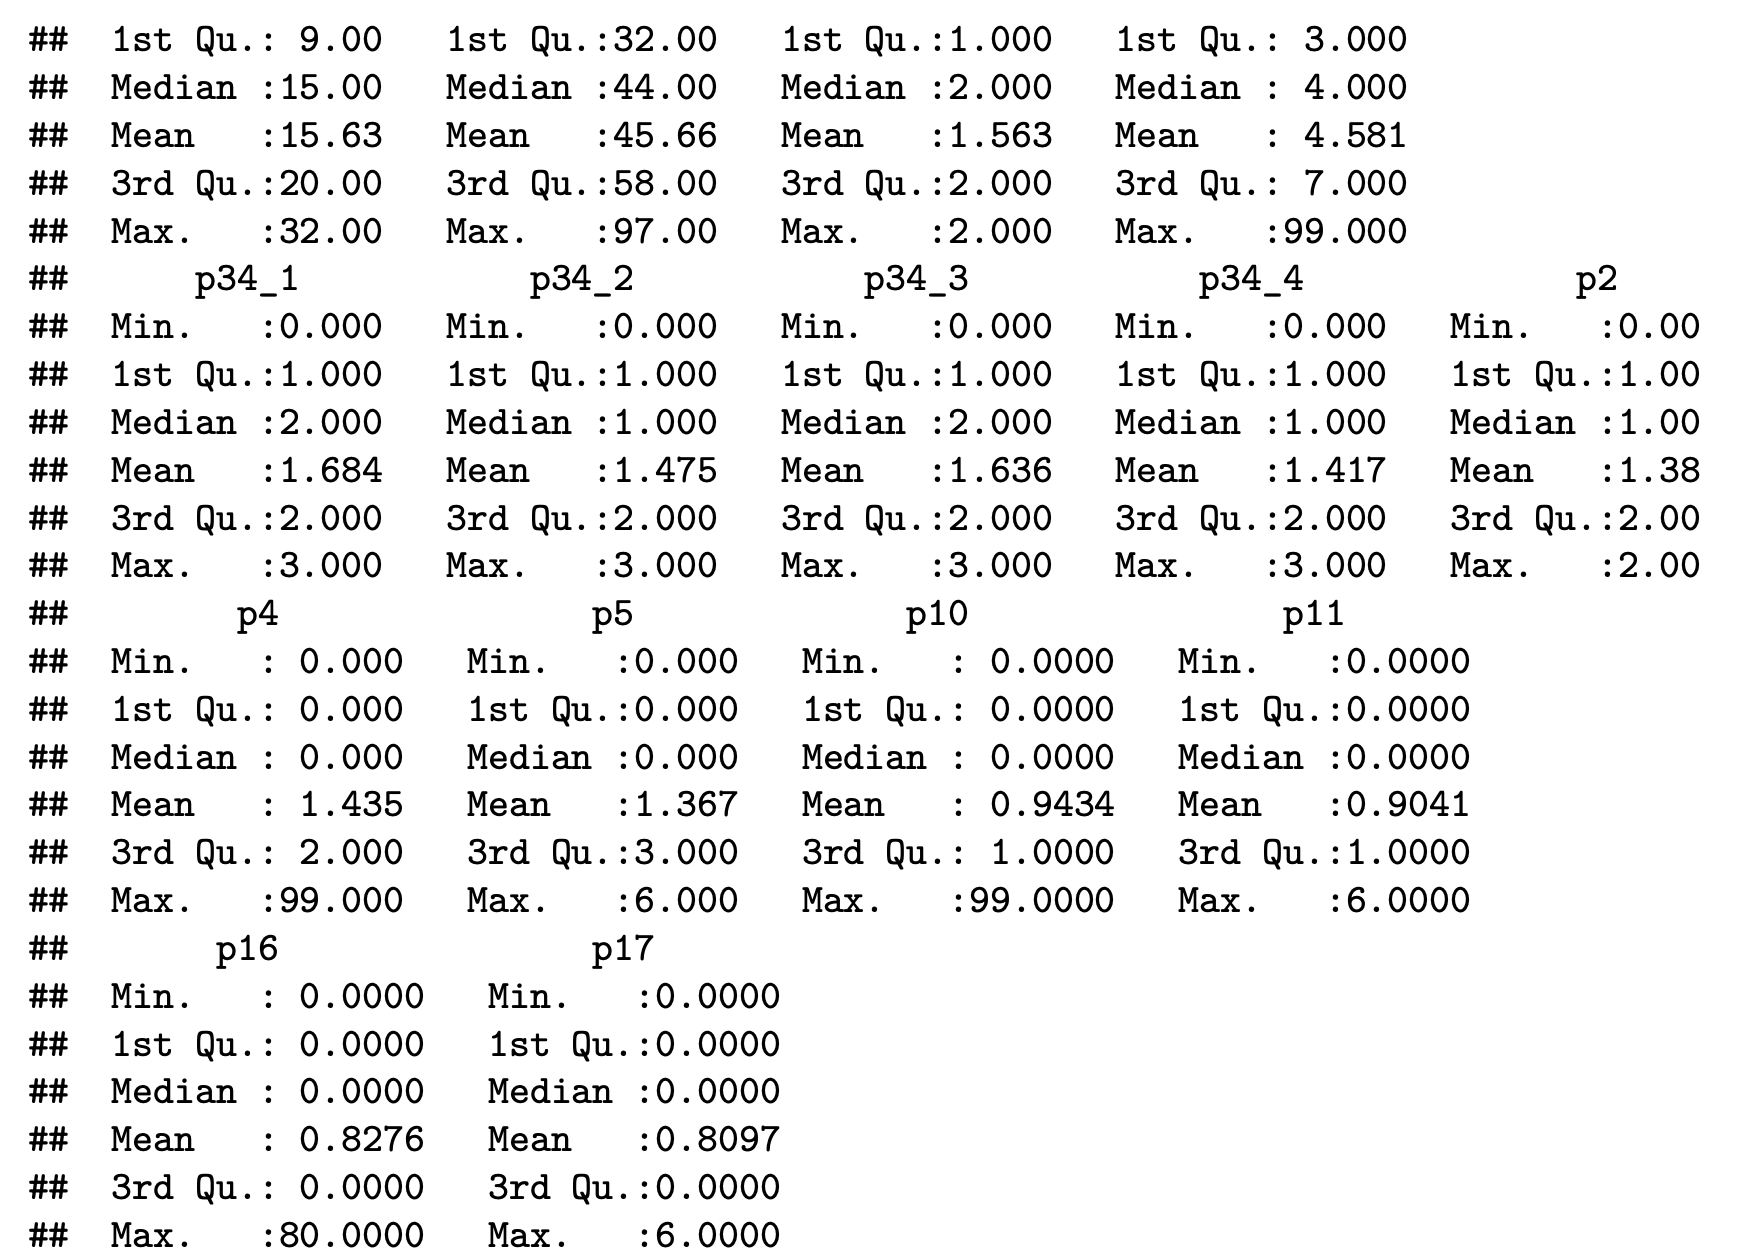
\includegraphics[width=0.8\textwidth]{Screenshot 2025-10-25 at 18.13.22.png}
  \label{fig:example_image}
  
\end{figure}
\end{widetext}

De aqui no se encontraron valores discrepantes.

\subsection{Valores vacios}

\begin{widetext}
\begin{figure}[H]
  \centering
  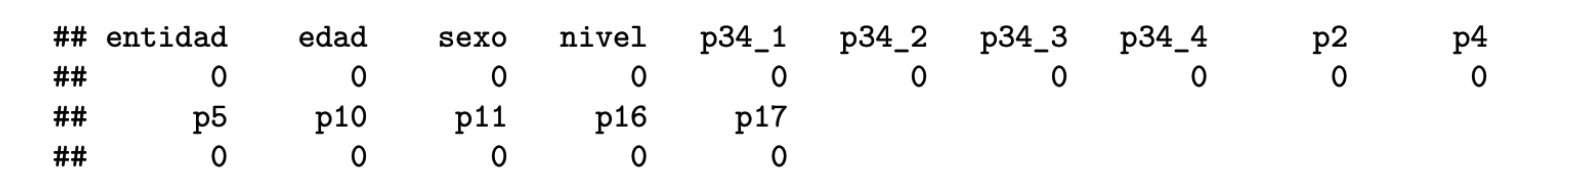
\includegraphics[width=0.8\textwidth]{Screenshot 2025-10-25 at 18.20.32.png}
\end{figure}
\end{widetext}

\subsection{Combinacion de columnas de textos leidos a TL}

\begin{widetext}
\begin{figure}[H]
  \centering
  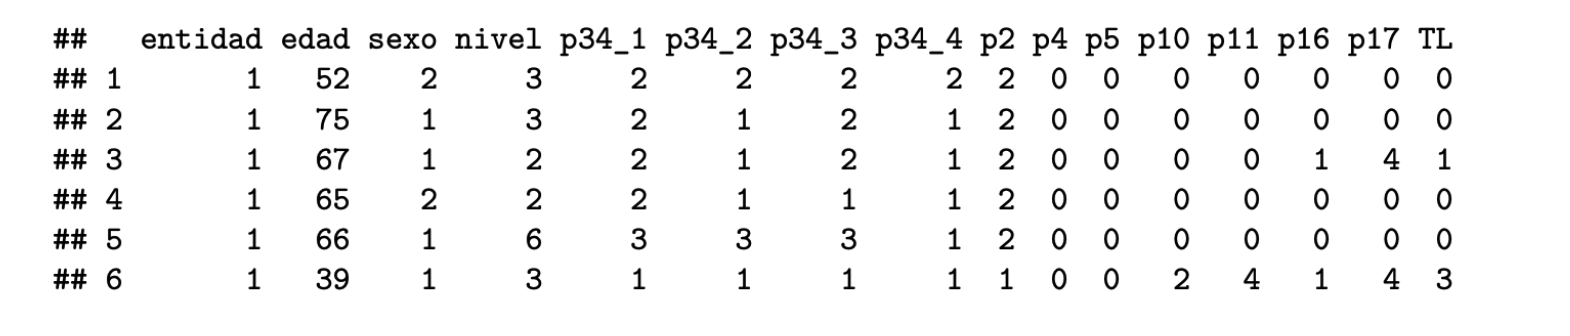
\includegraphics[width=0.8\textwidth]{Screenshot 2025-10-25 at 18.23.59.png}
\end{figure}
\end{widetext}

Se concluyó que no hubo necesidad de limpieza de datos y no mas que su preparación.

\section{Tablas de frecuencias}\label{tab_frec}
\begin{longtable}{ccc}
\caption{Tabla de Frecuencias: ENTIDAD (primeros 10 de 32)} \\
\toprule
\textbf{Código de Entidad} & \textbf{Frecuencia} & \textbf{Porcentaje (\%)} \\
\midrule
\endfirsthead

\multicolumn{3}{c}%
{{\bfseries \tablename\ \thetable{} -- continuación}} \\
\toprule
\textbf{Código de Entidad} & \textbf{Frecuencia} & \textbf{Porcentaje (\%)} \\
\midrule
\endhead



\bottomrule
\endlastfoot

1 & 275 & 2.30 \\
2 & 235 & 1.96 \\
3 & 217 & 1.81 \\
4 & 207 & 1.73 \\
5 & 286 & 2.39 \\
6 & 266 & 2.22 \\
7 & 254 & 2.12 \\
8 & 230 & 1.92 \\
9 & 1327 & 11.09 \\
10 & 257 & 2.15 \\
11 & 437 & 3.65 \\
12 & 261 & 2.18 \\
13 & 245 & 2.05 \\
14 & 1318 & 11.01 \\
15 & 885 & 7.40 \\
16 & 211 & 1.76 \\
17 & 255 & 2.13 \\
18 & 271 & 2.26 \\
19 & 1279 & 10.69 \\
20 & 267 & 2.23 \\
21 & 325 & 2.72 \\
22 & 256 & 2.14 \\
23 & 242 & 2.02 \\
24 & 240 & 2.01 \\
25 & 243 & 2.03 \\
26 & 242 & 2.02 \\
27 & 219 & 1.83 \\
28 & 256 & 2.14 \\
29 & 198 & 1.65 \\
30 & 305 & 2.55 \\
31 & 240 & 2.01 \\
32 & 217 & 1.81 \\
\end{longtable}

\begin{table}[h!]
\centering
\caption{Tabla de Frecuencias: P34\_1 (¿Llevaban a bibliotecas?)}
\begin{tabular}{lcc}
\toprule
\textbf{Categoría} & \textbf{Frecuencia} & \textbf{Porcentaje (\%)} \\
\midrule
Sí & 3456 & 29.58 \\
No & 7995 & 68.42 \\
No recuerda & 234 & 2.00 \\
\bottomrule
\end{tabular}
\end{table}

\begin{table}[h!]
\centering
\caption{Tabla de Frecuencias: P34\_2 (¿Veía a sus padres o tutores leer?)}
\begin{tabular}{lcc}
\toprule
\textbf{Categoría} & \textbf{Frecuencia} & \textbf{Porcentaje (\%)} \\
\midrule
Sí & 5907 & 50.55 \\
No & 5593 & 47.86 \\
No recuerda & 185 & 1.58 \\
\bottomrule
\end{tabular}
\end{table}

\begin{table}[h!]
\centering
\caption{Tabla de Frecuencias: P34\_3 (¿Sus padres o tutores le leían en voz alta?)}
\begin{tabular}{lcc}
\toprule
\textbf{Categoría} & \textbf{Frecuencia} & \textbf{Porcentaje (\%)} \\
\midrule
Sí & 5907 & 50.55 \\
No & 5593 & 47.86 \\
No recuerda & 185 & 1.58 \\
\bottomrule
\end{tabular}
\end{table}
\begin{table}[h!]
\centering
\caption{Tabla de Frecuencias: P11 (Motivo de lectura de revistas)}
\begin{tabular}{lcc}
\toprule
\textbf{Categoría} & \textbf{Frecuencia} & \textbf{Porcentaje (\%)} \\
\midrule
Trabajo & 281 & 9.01 \\
Estudio & 147 & 4.71 \\
Cultura general & 739 & 23.69 \\
Gusto/Entretenimiento & 1747 & 56.01 \\
Religión & 192 & 6.16 \\
Otro & 13 & 0.42 \\
\bottomrule
\end{tabular}
\end{table}

\begin{table}[h!]
\centering
\caption{Tabla de Frecuencias: P17 (Motivo de lectura de periódicos)}
\begin{tabular}{lcc}
\toprule
\textbf{Categoría} & \textbf{Frecuencia} & \textbf{Porcentaje (\%)} \\
\midrule
Trabajo & 80 & 2.72 \\
Estudio & 34 & 1.16 \\
Cultura general & 1799 & 61.17 \\
Gusto/Entretenimiento & 1009 & 34.31 \\
Religión & 6 & 0.20 \\
Otro & 13 & 0.44 \\
\bottomrule
\end{tabular}
\end{table}

\section{Gráficas}\label{graficas}

\begin{figure}[H]
  \centering
  \includegraphics[width=0.4\textwidth]{Screenshot 2025-10-25 at 19.43.27.png}
  \caption{Densidad de textos leidos}
\end{figure}

\begin{figure}[H]
  \centering
  \includegraphics[width=0.4\textwidth]{Screenshot 2025-10-25 at 19.44.10.png}
  \caption{Grafico de caja de relacion entre textos leidos y edad}
\end{figure}

\begin{figure}[H]
  \centering
  \includegraphics[width=0.4\textwidth]{Screenshot 2025-10-25 at 19.44.55.png}
  \caption{Personas que fueron a una libreria en su infancia}
\end{figure}

\begin{figure}[H]
  \centering
  \includegraphics[width=0.4\textwidth]{Screenshot 2025-10-25 at 19.46.19.png}
  \caption{Análisis de dispersion de  personas que fueron llevadas a bibliotecas y su cantidad de textos leidos.}
\end{figure}

\begin{figure}[H]
  \centering
  \includegraphics[width=0.4\textwidth]{Screenshot 2025-10-25 at 19.47.51.png}
  \caption{Grafico de barras de cantidad de personas que acostumbran leer}
\end{figure}

\section{Intervalos de confianza}\label{int_conf}

\begin{lstlisting}
## 1) Proporción P5 ='Gusto/Entretenimiento'
## n = 4868 k = 2060
## p = 0.4232 IC 96% = [ 0.4086 , 0.4377 ]
## 2) Diferencia de proporciones (Libros en casa: Sí vs No)
## n(Sí) = 3591 k(Sí) = 1532 p1 = 0.4266
## n(No) = 1205 k(No) = 501 p2 = 0.4158
## p1 - p2 = 0.0109 IC 96% = [ -0.0229 , 0.0446 ]
## 3) Media TL (total leído)
## n = 11966 media = 3.2057 sd = 6.028
## IC 96% (t) = [ 3.0925 , 3.3189 ]
13
## 4) Varianza p4 (número de libros leídos)
## n = 11966 s^2 = 14.8427
## IC 96% para ^2 = [ 14.4562 , 15.2447 ]
\end{lstlisting}


\nocite{*}
\bibliography{references.bib}

\end{document}